\documentclass{article}

\usepackage{assumptionsofphysics}
\usepackage{tikz}
\usetikzlibrary{shapes,snakes}
\usepackage{hyperref}
\hypersetup{
	colorlinks=true,
	citecolor=blue,
	urlcolor=blue,
	linkcolor=blue
}
\frenchspacing

\newcommand{\marginleft}[1] {\reversemarginpar\marginpar{#1}}
\newcommand{\marginright}[1] {\normalmarginpar\marginpar{#1}}

\title{Bare minimum: set theory}

\date{\vspace{-5ex}}
\begin{document}

\maketitle


\begin{abstract}
This note presents a condensed summary of set theory which can function as a crash course, refresher and/or reference. Bare minima are meant to give a rough overview, by no means complete, of the subject to the intellectually curious, particularly in the context of foundational questions in physics. This work is part of Assumptions of Physics (\url{https://assumptionsofphysics.org}), a project that aims to identify a handful of physical principles from which the basic laws can be rigorously derived.
\end{abstract}

\section{Introduction}

Set theory is important for those working on the Assumptions of Physics for at least three reasons. First, it is a foundational framework in mathematics. Second, it showcases a successful attempt at concept generalization. Third, it shows how a formal system is bootstrapped.

There are two rough branches of set theory: naive and axiomatic. Naive set theory is built on intuitive concepts, and as such is not fully formalized and is open to potential paradoxes. Axiomatic set theory provides a fully formalized axiomatic system that aims to close those problems. We will start with naive set theory, which is the best setting for defining all the basic notions and getting a sense of how the framework works. Then we will turn our attention to axiomatic set theory to get a sense of what problems it solves and how, and whether those solutions mesh with foundational goals  in physics.

TODO: cite https://www.math24.net/topics-set-theory and set theory book

\section{Naive set theory}

We take sets and elements as primitive objects, with no formal definition. A \textbf{set} $A$ is a collection of elements. If an element $e$ belongs to the set we say $e$ \textbf{is in} $A$, noted $ e 
\in A$. A set $A$ can be defined by listing the elements, noted $A = \{ e_1, e_2, e_3 \}$. A set $A$ can be defined by specifying how to build the elements through a rule (i.e. predicate) $P(e)$, and is noted $A = \{e \, | \,  P(e) \}$. The rule may include symbols like for all $\forall$, exists $\exists$, logical connectors AND $\AND$, OR $\OR$ and $\NOT$.

\begin{defn}[Common sets]
	 The \textbf{empty set}
	 \marginleft{Common sets: $\emptyset$, $\mathbb{N}$, $\mathbb{Z}$, $\mathbb{R}$, $\mathbb{C}$}
	  $\emptyset$ is the set with no elements.
	 The \textbf{set of natural numbers} $\mathbb{N} = \{ 0, 1, 2, ... \}$. The \textbf{set of positive natural numbers} $\mathbb{N}^+ = \{n \in \mathbb{N} \, | \, n > 0\}$. The \textbf{set of integer numbers} $\mathbb{Z} = \{ ... , -2, -1, 0, +1, +2, ...\}$. The \textbf{set of rational numbers} $\mathbb{Q}$. The \textbf{set of real numbers} $\mathbb{R}$. The \textbf{set of complex numbers} $\mathbb{C}$. A \textbf{universe} $U$ is the set that, within a specific context, contains all entities under study.
\end{defn}

\subsection{Basic definitions}

\begin{defn}[Set relationships]
	Let $A$ and $B$ be two sets. \marginleft{Subset, superset: $\subseteq$, $\supseteq$} If all elements in $A$ are also contained in $B$, we say $A$ is a \textbf{subset} of $B$, noted $A \subseteq B$. In this case, we also say $B$ is a \textbf{superset} of $A$, noted $B \supseteq A$. Additionally, if $B$ contains elements that $A$ does not contain, we say $A$ is a \textbf{strict subset} of $B$, noted $A \subset B$, and $B$ is a \textbf{strict superset} of $A$, noted $B \supset A$. If the two sets contain exactly the same elements, then we say the sets are \textbf{equal}, noted $A = B$. If the two sets have no element in common they are said to be \textbf{disjoint}.
\end{defn}

\begin{defn}[Power set]
	Given a set $A$, its \textbf{power set}, \marginleft{Power set: $2^{A}$, $\mathcal{P}(A)$} noted $\mathcal{P}(A)$ or $2^{A}$, is the set of all subsets of $A$. That is, $\mathcal{P}(A) = \{B \, | \, B \subset A \}$.
\end{defn}

\begin{defn}[Set operations]
	We define \marginleft{Set operations: $\cup$, $\cap$, $\setminus$, $^{\complement}$} the following operations between two sets $A$ and $B$:
	\begin{description}
		\item[Union.]Noted $A \cup B$, the union of $A$ and $B$ is the set of all elements that are contained by $A$, $B$ or both.
		\marginright{
			\def\setA{ (-1,0) circle (2) }
			\def\setB{ (1,0) circle (2) }
			\begin{tikzpicture}[scale = 0.3]
				\filldraw[black!10] \setA;
				\filldraw[black!10] \setB;
				\draw \setA; 
				\draw \setB;
				\node at (-4.7,0) {$A\!\cup \! B$};
			\end{tikzpicture} 
			\begin{tikzpicture}[scale = 0.3]
				\begin{scope}
					\clip \setA;
					\filldraw[black!10] \setB;
				\end{scope}
				\draw \setA; 
				\draw \setB;
				\node at (-4.7,0) {$A\!\cap \! B$};
			\end{tikzpicture} 
			\begin{tikzpicture}[scale = 0.3]
				\filldraw[black!10] \setA;
				\filldraw[white] \setB;
				\draw \setA; 
				\draw \setB;
				\node at (-4.7,0) {$A\!\setminus \! B$};
			\end{tikzpicture} 
			\def\setU{ (-3,-2) rectangle (3,2) }
			\def\setA{ (0,0) circle (1.8) }
			\begin{tikzpicture}[scale = 0.3] 
				\filldraw[black!10] \setU;
				\filldraw[white] \setA;
				\draw \setU;
				\draw \setA;
				\node at (-5.3,0) {$A^{\complement}$};
			\end{tikzpicture} 
		}\item[Intersection.] Noted $A \cap B$, the intersection of $A$ and $B$ is the set of all elements that are contained by both.
		\item[Set difference (or relative complement).] Noted $A \setminus B$, $A$ minus $B$ is the set of all elements in $A$ that are not contained by $B$.
		\item[Complement (or absolute complement).] Noted $A^{\complement}$, represents all elements that are not contained in $A$. Note that this operation is context specific: we need to know that, within a certain context, $U$ is the set of all elements under study; then the complement of $A \subseteq U$ is $A^{\complement} = U \setminus A$.
	\end{description}
\end{defn}


We give the following informal definition. Given two elements $a$ and $b$, the \textbf{ordered pair} $(a, b)$ specifies two objects in that order. That is $(a, b) \neq (b, a)$ and $(a, a) \neq \{a\}$.

\marginright{~\\
	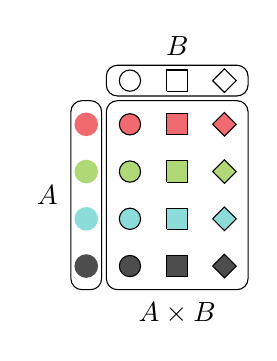
\begin{tikzpicture}[scale = 0.3] 
		\node at (-2.5,-4) {$A$};
		\node at (3,2.3) {$B$};
		\draw[rounded corners] (0,0.2) rectangle (6,1.5);
		\draw[rounded corners] (-0.2,0) rectangle (-1.5,-8);
		\draw[rounded corners] (0,0) rectangle (6,-8);
		
		\def\circlepath{circle (0.45)}
		\def\rectanglepath{ ++(-0.45,-0.45)  -- ++(0,0.9)  -- ++(0.9,0) -- ++(0,-0.9) -- ++(-0.9,0)}
		\def\diamondpath{ ++(-0.5,0)  -- ++(0.5,0.5)  -- ++(0.5,-0.5) -- ++(-0.5,-0.5) -- ++(-0.5,0.5)}
		
		% B elements
		\draw (1,0.85) \circlepath;
		\draw (3,0.85) \rectanglepath;
		\draw (5,0.85) \diamondpath;
		
		\definecolor{a}{rgb}{0.945, 0.415, 0.439}
		\definecolor{b}{rgb}{0.694, 0.847, 0.466}
		\definecolor{c}{rgb}{0.549, 0.862, 0.854}
		\definecolor{d}{rgb}{0.301, 0.301, 0.301}
		
		% A elements
		\fill[a] (-0.85, -1) circle (0.5);
		\fill[b] (-0.85, -3) circle (0.5);
		\fill[c] (-0.85, -5) circle (0.5);
		\fill[d] (-0.85, -7) circle (0.5);

		% AxB elements
		\filldraw[fill=a] (1, -1) \circlepath;
		\filldraw[fill=b] (1, -3) \circlepath;
		\filldraw[fill=c] (1, -5) \circlepath;
		\filldraw[fill=d] (1, -7) \circlepath;
		\filldraw[fill=a] (3, -1) \rectanglepath;
		\filldraw[fill=b] (3, -3) \rectanglepath;
		\filldraw[fill=c] (3, -5) \rectanglepath;
		\filldraw[fill=d] (3, -7) \rectanglepath;
		\filldraw[fill=a] (5, -1) \diamondpath;
		\filldraw[fill=b] (5, -3) \diamondpath;
		\filldraw[fill=c] (5, -5) \diamondpath;
		\filldraw[fill=d] (5, -7) \diamondpath;

		\node at (3,-9) {$A \times B$};
	\end{tikzpicture} 
}
\begin{defn}[Cartesian product]
	Given two sets \marginleft{Cartesian product: $\times$}  $A$ and $B$, the \textbf{Cartesian product} $A \times B = \{ (a,b) \, | \, \forall a \in A, b \in B \}$ is the set of all possible ordered pairs between the elements of $A$ and $B$.
\end{defn}

\subsection{Relations and function}

\begin{remark}
	Relations provide a common foundation for functions (i.e. the relation is the set of pairs $(x, f(x))$), equivalences and order (i.e. the relation is the set of pairs $(a, b)$ such that $a=b$ or $a\leq b$ respectively). This is an example of highly fruitful generalization.
\end{remark}

\begin{defn}[Binary relation]
	Given a set $A$, called \textbf{domain}, and a set $B$, called \textbf{codomain}, a \textbf{binary relation} is a set $R \subseteq A \times B$ of ordered pairs. We say $a$ is \textbf{$R$-related} to $b$, noted $aRb$ if $(a,b) \in R$. If $A=B$ (i.e. domain and codomain coincide) the relation is said \textbf{homogeneous}, \textbf{heterogeneous} if not.
\end{defn}
	
\begin{defn}[Image and preimage]
	If $X \subseteq A$, the \textbf{image of $X$ under $R$} is the set of all elements in $B$ that are related to at least one element in $X$. The \textbf{image of $R$} is set of all elements in $B$ that are related to at least one element in $A$ (i.e. the image of the full set $A$).
	
	If $Y \subseteq B$, the \textbf{preimage of $Y$ under $R$} is the set of all elements in $A$ that are related to at least one element in $Y$. The \textbf{preimage of $R$} is set of all elements in $A$ that are related to at least one element in $B$ (i.e. the preimage of the full set $B$).
\end{defn}

\begin{defn}
	Given a relationship $R$ between $A$ and $B$, the \textbf{converse} or \textbf{inverse} relationship $R^{-1}$ is the relationship where the order of the pairs is inverted. That is, $R^{-1} = \{ (b, a) \, | \, (a, b) \in R\}$.
\end{defn}

\begin{defn}[Relation properties]
	Let $R$ be a binary relation between $A$ and $B$. We define the following properties:
	\begin{description}
		\item[Functional or right-unique.] An element $a \in A$ is related to at most one element $b \in B$. That is, if $aRb$ and $cRb$ then $a = c$.
		\item[Injective or left-unique.] An element $b \in B$ is related to at most one element $a \in A$. That is, if $aRb$ and $aRc$ then $b = c$.
		\item[Serial or left-total.] Every element $a \in A$ is related to at least one element $b \in B$. That is, for each $a \in A$ there exists at least one $b \in B$ such that $aRb$. In this case, the preimage of $R$ is the whole $A$.
		\item[Surjective or right-total.] Every element $b \in B$ is related to at least one element $a \in B$. That is, for each $b \in B$ there exists at least one $a \in A$ such that $aRb$. In this case, the image of $R$ is the whole $B$.
	\end{description}
	From those basic properties, we define the following:
	\begin{description}
		\item[One-to-one.] Injective and functional (i.e. left-unique and right-unique).
		\item[One-to-many.] Injective and not functional (i.e. left-unique and not right-unique).
		\item[Many-to-one.] Not injective and functional (i.e. not left-unique and right-unique).
		\item[Many-to-many.] Not injective nor functional (i.e. not left-unique nor right-unique).
	\end{description}	
\end{defn}

\begin{defn}[Function]
	A \textbf{partial function} $f : A \to B$ is a binary relationship between $A$ and $B$ that is functional (i.e. right-unique). The \textbf{graph} of the function $G \subset A \times B$ is the function expressed as ordered pairs. A \textbf{total function}, or simply a \textbf{function}, is a partial function that is also serial (i.e. left-total, defined on the whole domain). A function is \textbf{bijective} if it is injective and surjective.
	
	When the functional form $f(a)$ is known, this can be expressed as $a \mapsto f(a)$ (read ``$a$ maps to $f$ of $a$'').
\end{defn}

\begin{remark}
	Note that the domain and the codomain can be any set, including scalar products. Therefore $f : \mathbb{R} \times \mathbb{R} \to \mathbb{R}$ for which $(x,y) \mapsto \sqrt{x^2 + y^2}$ gives us the Euclidean norm of a two dimensional vector.
\end{remark}

\begin{defn}[Identity function]
	Given a set $A$, the identity function $\Id_A : A \to A$ is the function such that $\Id_A(a) = a$ for all $a \in A$.
\end{defn}


\marginpar[Left]{Right}
\begin{prop}[Inverse function]
	Let $f : A \to B$ be a function. The corresponding converse relationship $f^{-1}$ is a function if and only if $f$ is bijective. In this case $f^{-1} : B \to A$ is also bijective and is called the \textbf{inverse} of $f$.
\end{prop}

\begin{defn}[Composition]
	Let $A$, $B$ and $C$ be three sets. Let $R$ be a binary relationship between $A$ and $B$ and $S$ be a binary relationship between $B$ and $C$. Then the \textbf{composition of $R$ and $S$}, noted $S \circ R$, is the binary relationship between $A$ and $C$ such that $(a, c) \in S \circ R$ if we can find $b \in B$ such that $aRb$ and $bSc$.
\end{defn}

\begin{remark}
	The order of composition follows those of functions: if $f : A \to B$ and $g : B \to C$, composition leads to $c = g(f(a)) = (g \circ f)(a)$.
\end{remark}

\begin{prop}[Composition properties]
	Relation composition follows the following properties:
	\begin{itemize}
		\item Composition is associative: $R \circ (T \circ S) = (R \circ T) \circ S$
		\item Converse of composition: $(R \circ S)^{-1} = S^{-1} \circ R^{-1}$
		\item Composition of functional/injective/serial/surjective relations is \\ functional/injective/serial/surjective.
		\item If $f : A \to B$ and $g : B \to C$ are (partial) functions, then $g \circ f$ is a (partial) function.
		\item Let $f : A \to B$ is a bijective function, then $f \circ f^{-1} = \Id_B$ and $f^{-1} \circ f = \Id_A$.
	\end{itemize}
\end{prop}

\begin{defn}[Sets of functions]
	The set of all possible functions $f : A \to B$ is noted $B^A$.
\end{defn}

\begin{remark}
	The notation is due to the cardinality. If $|A| = n$ and $|B| = m$, each function is given by choosing an element of $B$ for each element of $A$, that is $m$ choices $n$ times, that is $m^n$. The power set is noted $2^A$ because each subset can be identified by a function $U : A \to \{0 , 1\}$, where $f(a)=0$ corresponds to $a \notin U$ and $f(a)=0$ corresponds to $b \in U$.
\end{remark}

\subsection{Indexed families and sequences}

\begin{defn}[Families]
	An \textbf{indexed family}, or simply a \textbf{family}, $\{x_i\}_{i \in I}$ is a collection of elements identified by an \textbf{index set} $I$. More formally, an indexed family is a tuple $\langle X, I, x \rangle$ where $X$ and $I$ are sets and $x: I \to X$ is a function such that $i \mapsto x_i$. A \textbf{sequence} is an family for which the index set is a continuous interval of natural numbers. A \textbf{finite sequence} of $n$ elements is noted $\{x_i\}_{i=1}^{n}$ while an \textbf{infinite sequence} is noted $\{x_i\}_{i=1}^{\infty}$.
\end{defn}

\begin{defn}[Operations on families of sets]
	Let $\{A_i\}_{i \in I}$ be a family of sets, the operations of intersection $\bigcap\limits_{i \in I} A_i $ and union $\bigcup\limits_{i \in I} A_i$ can be extended to span all members.
\end{defn}

\begin{defn}[Set-theoretic limit]
	Let $\{A_i\}_{i=0}^{\infty}$ be a sequence of sets. We define the \textbf{limit infimum} as $\liminf\limits_{i \to \infty} A_i = \bigcup\limits_{i \geq 1}\bigcap\limits_{j \geq i} A_j$ and the \textbf{limit supremum} as $\limsup\limits_{i \to \infty} A_i = \bigcap\limits_{i \geq 1}\bigcup\limits_{j \geq i} A_j$. If the two are equal to the same set then we say the sequence \textbf{converges}, the \textbf{set-theoretic limit} exists and it is equal to that set.
\end{defn}

\begin{defn}[Monotone sequence]
	A \textbf{monotone sequence} is a sequence of sets $\{A_i\}_{i=0}^{\infty}$ where each set is a superset (or subset) of the preceding. More specifically, we distinguish four cases:
	\begin{description}
		\item[Increasing] when $A_i \subseteq A_{i+1}$ for all $i>0$
		\item[Decreasing] when $A_i \supseteq A_{i+1}$ for all $i>0$
		\item[Strictly increasing] when $A_i \subset A_{i+1}$ for all $i>0$
		\item[Strictly decreasing] when $A_i \supset A_{i+1}$ for all $i>0$
	\end{description}
\end{defn}

\begin{prop}
	All monotone sequences converge. For increasing sequences the limit is given by $\lim\limits_{i \to \infty} A_i = \bigcup\limits_{i \geq 1} A_i$, while for decreasing sequences  the limit is given by $\lim\limits_{i \to \infty} A_i = \bigcap\limits_{i \geq 1} A_i$.
\end{prop}

\subsection{Homogeneous relations, equivalences and orders}

\subsection{Numeric constructions}
\begin{remark}
	The constructions that follow exemplifies the standard way numbers are defines in mathematics and it is useful to gain certain insights. In the Assumptions of Physics, however, we prefer to understand numbers as order-theoretic concept (i.e. the integer numbers can be thought as a linearly ordered set where each element have an immediate successor and an immediate predecessor).
\end{remark}
\begin{defn}
	Let $A$ be a set. We define the \textbf{successor} $A^+ = A \cup \{A\}$. A set $S$ is called a \textbf{successor set} if it contains the empty set (i.e. $\emptyset \in S$ and if contains the successor of every element (i.e. if $X \in S$ then $X^+ \in S$). The set of \textbf{natural numbers} $\mathbb{N}$ is the intersection of all successor sets.
\end{defn}
\begin{remark}
	The natural numbers so constructed are known as von Neumann ordinals. They are as follows:
	\begin{itemize}
		\item $0 = \{ \} = \emptyset$
		\item $1 = \{ 0 \} = \{ \emptyset \}$
		\item $2 = \{0, 1\} = \{ \emptyset, \{ \emptyset\} \}$
		\item $3 = \{0, 1, 2\} = \{ \emptyset, \{ \emptyset\}, \{ \emptyset, \{ \emptyset\} \} \}$
		\item $4 = \{0, 1, 2, 3\} = \{ \emptyset, \{ \emptyset\}, \{ \emptyset, \{ \emptyset\} \}, \{ \emptyset, \{ \emptyset\}, \{ \emptyset, \{ \emptyset\} \} \} \}$
		\item ...
	\end{itemize}
\end{remark}

\section{Axiomatic set theory}

Introduce paradoxes. Axiomatic set theory is a family of attempt to solve those paradoxes. There are different variations.

Formalization to remove semantic paradoxes. All approaches of axiomatic set theory do that.

%https://en.wikipedia.org/wiki/Zermelo%E2%80%93Fraenkel_set_theory

%https://en.wikipedia.org/wiki/Von_Neumann–Bernays–Gödel_set_theory

Syntactic paradoxes two main strategies. Zermelo–Fraenkel (ZFC) only talk about sets and restrict set construction to subsets only. von Neumann–Bernays–Gödel (NBG) talks about classes and defines sets as those classes that can be elements of classes. Set builder notation works on sets, not classes. So, if putting a class in a class creates a contradiction, it's because the class is not a set, but a proper class.

Ugly elements of set theory: all mathematical objects are sets. Numbers are set.

%\bibliographystyle{plain}
%\bibliography{bibliography}

\end{document}